\chapter*{Proposition 47}



\begin{figure*}[ht]
    \begin{center}
    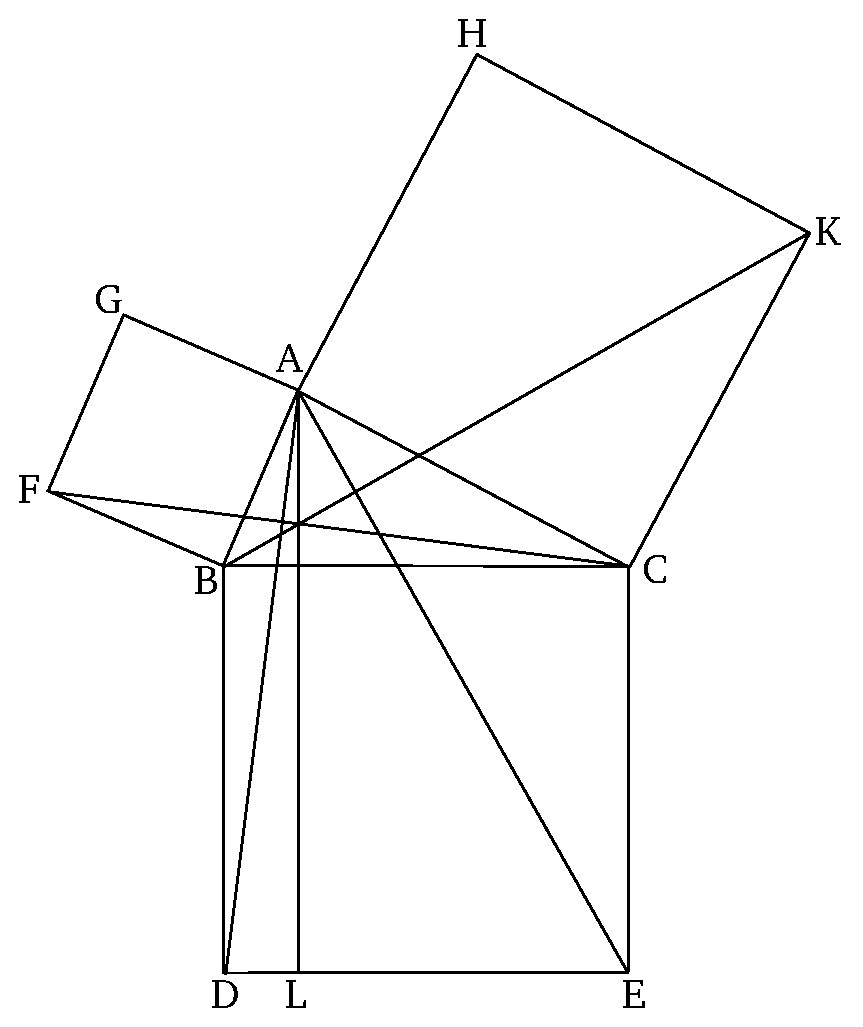
\includegraphics[width=0.5\linewidth]{figures/fig47e.eps}
    \label{fig:prop_47}
    \end{center}
\end{figure*}

In right-angled triangles,  the square on the side subtending the right-angle
is equal to the (sum of the) squares on the sides containing the right-angle.

Let $ABC$ be a right-angled triangle having the angle $BAC$a right-angle. I say that the
square on $BC$ is equal to the (sum of the) squares on $BA$ and $AC$.

For let the square $BDEC$ have been described on $BC$, and (the squares) $GB$ and $HC$ on $AB$ and $AC$ (respectively) [Prop.~1.46]. And let $AL$ have been drawn through point $A$ parallel to either of $BD$ or $CE$ [Prop.~1.31]. And let $AD$ and $FC$ have been joined. And
since angles $BAC$ and $BAG$ are each right-angles, then two straight-lines $AC$ and $AG$, not lying on the same side,
make the adjacent angles with some straight-line $BA$, at the point
$A$ on it, (whose sum is) equal to two right-angles. Thus, $CA$ is straight-on to $AG$ [Prop.~1.14]. So, for
the same (reasons), $BA$ is also straight-on to $AH$. And since angle $DBC$ is
equal to $FBA$, for (they are) both right-angles, let $ABC$ have been added to
both.  Thus, the whole (angle) $DBA$ is equal to the whole (angle) $FBC$.
And since $DB$ is equal to $BC$, and $FB$ to $BA$, the two (straight-lines) $DB$,
$BA$ are equal to the two (straight-lines) $CB$, $BF$,$^\dag$ respectively. And angle $DBA$ (is) equal to angle $FBC$. Thus, the base $AD$ [is] equal to the base $FC$,
and the triangle $ABD$ is equal to the triangle $FBC$ [Prop.~1.4]. And 
parallelogram $BL$ [is] double (the area) of triangle $ABD$. For they
have the same base, $BD$, and are between the same parallels, $BD$ and $AL$  [Prop.~1.41]. And
 square
$GB$ is double (the area) of triangle $FBC$. For again they have the same base, $FB$, and
are between the same parallels,
$FB$ and $GC$ [Prop.~1.41]. [And the doubles of equal things
are equal to one another.]$^\ddag$ Thus, the parallelogram $BL$ is also equal to the square $GB$. So, similarly, $AE$ and $BK$ being joined, 
the parallelogram $CL$ can be shown (to be)  equal to the square $HC$. Thus, the whole square
$BDEC$ is equal to the (sum of the) two squares $GB$ and $HC$. And the square $BDEC$
is described on $BC$, and the (squares) $GB$ and $HC$ on $BA$ and $AC$ (respectively). Thus, the square on the side $BC$ is equal to the
(sum of the) squares
on the sides $BA$ and $AC$.

Thus, in right-angled triangles,  the square on the side subtending the right-angle
is equal to the (sum of the) squares on the sides surrounding the right-[angle].
(Which is) the very thing it was required to show.


\section*{Commentary}

\begin{proposition}\label{proposition_47}\lean{Elements.Book1.proposition_47}\leanok
    If
\end{proposition}
\begin{proof}
    \uses{proposition_4,proposition_13,proposition_14,proposition_16,proposition_17,proposition_30,proposition_31,proposition_41,proposition_46}\leanok
\end{proof}
